\documentclass{standalone}
\usepackage{tikz}
\usetikzlibrary{patterns}
\usetikzlibrary{positioning}
\usetikzlibrary{patterns, positioning}
\usetikzlibrary{shapes.misc}
\usepackage[outline]{contour}
\contourlength{1.5pt} 


\begin{document}
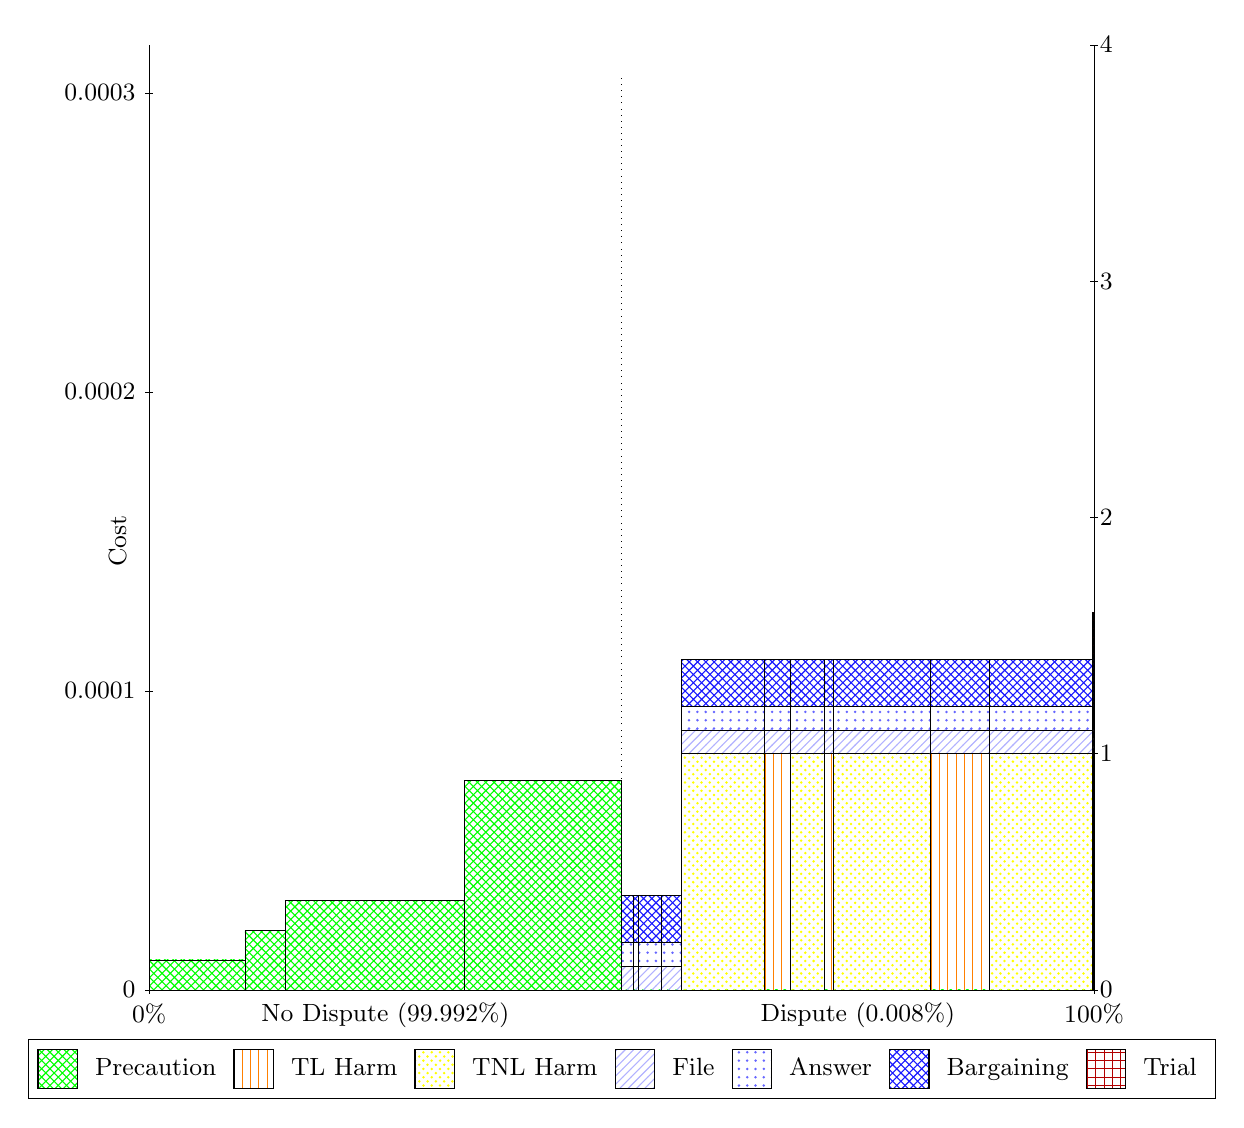
\begin{tikzpicture}
\draw[pattern=crosshatch, pattern color=green,draw=black,very thin] (1.5,2.5) rectangle (2.7156,2.8797);
\draw[pattern=crosshatch, pattern color=green,draw=black,very thin] (2.7156,2.5) rectangle (3.2309,3.2594);
\draw[pattern=crosshatch, pattern color=green,draw=black,very thin] (3.2309,2.5) rectangle (5.5,3.6391);
\draw[pattern=crosshatch, pattern color=green,draw=black,very thin] (5.5,2.5) rectangle (7.5,5.158);
\draw[pattern=crosshatch, pattern color=green,draw=black,very thin] (7.5,2.5) rectangle (7.6515,2.5);
\draw[pattern=north east lines, pattern color=blue!30,draw=black,very thin] (7.5,2.5) rectangle (7.6515,2.8);
\draw[pattern=dots,  pattern color=blue!60,draw=black,very thin] (7.5,2.8) rectangle (7.6515,3.1);
\draw[pattern=crosshatch,      pattern color=blue!90,draw=black,very thin] (7.5,3.1) rectangle (7.6515,3.7);
\draw[pattern=crosshatch, pattern color=green,draw=black,very thin] (7.6515,2.5) rectangle (7.7163,2.5001);
\draw[pattern=north east lines, pattern color=blue!30,draw=black,very thin] (7.6515,2.5001) rectangle (7.7163,2.8001);
\draw[pattern=dots,  pattern color=blue!60,draw=black,very thin] (7.6515,2.8001) rectangle (7.7163,3.1001);
\draw[pattern=crosshatch,      pattern color=blue!90,draw=black,very thin] (7.6515,3.1001) rectangle (7.7163,3.7001);
\draw[pattern=crosshatch, pattern color=green,draw=black,very thin] (7.7163,2.5) rectangle (8.0035,2.5001);
\draw[pattern=north east lines, pattern color=blue!30,draw=black,very thin] (7.7163,2.5001) rectangle (8.0035,2.8001);
\draw[pattern=dots,  pattern color=blue!60,draw=black,very thin] (7.7163,2.8001) rectangle (8.0035,3.1001);
\draw[pattern=crosshatch,      pattern color=blue!90,draw=black,very thin] (7.7163,3.1001) rectangle (8.0035,3.7001);
\draw[pattern=crosshatch, pattern color=green,draw=black,very thin] (8.0035,2.5) rectangle (8.2567,2.5002);
\draw[pattern=north east lines, pattern color=blue!30,draw=black,very thin] (8.0035,2.5002) rectangle (8.2567,2.8002);
\draw[pattern=dots,  pattern color=blue!60,draw=black,very thin] (8.0035,2.8002) rectangle (8.2567,3.1002);
\draw[pattern=crosshatch,      pattern color=blue!90,draw=black,very thin] (8.0035,3.1002) rectangle (8.2567,3.7002);
\draw[pattern=crosshatch, pattern color=green,draw=black,very thin] (8.2567,2.5) rectangle (8.2591,2.5);
\draw[pattern=north east lines, pattern color=blue!30,draw=black,very thin] (8.2567,2.5) rectangle (8.2591,2.8);
\draw[pattern=dots,  pattern color=blue!60,draw=black,very thin] (8.2567,2.8) rectangle (8.2591,3.1);
\draw[pattern=crosshatch,      pattern color=blue!90,draw=black,very thin] (8.2567,3.1) rectangle (8.2591,3.7);
\draw[pattern=grid,            pattern color=red!70!black,draw=black,very thin] (8.2567,3.7) rectangle (8.2591,4.3);
\draw[pattern=crosshatch, pattern color=green,draw=black,very thin] (8.2591,2.5) rectangle (9.3162,2.5);
\draw[pattern=crosshatch dots, pattern color=yellow,draw=black,very thin] (8.2591,2.5) rectangle (9.3162,5.5);
\draw[pattern=north east lines, pattern color=blue!30,draw=black,very thin] (8.2591,5.5) rectangle (9.3162,5.8);
\draw[pattern=dots,  pattern color=blue!60,draw=black,very thin] (8.2591,5.8) rectangle (9.3162,6.1);
\draw[pattern=crosshatch,      pattern color=blue!90,draw=black,very thin] (8.2591,6.1) rectangle (9.3162,6.7);
\draw[pattern=crosshatch, pattern color=green,draw=black,very thin] (9.3162,2.5) rectangle (9.6405,2.5);
\draw[pattern=vertical lines, pattern color=orange,draw=black,very thin] (9.3162,2.5) rectangle (9.6405,5.5);
\draw[pattern=north east lines, pattern color=blue!30,draw=black,very thin] (9.3162,5.5) rectangle (9.6405,5.8);
\draw[pattern=dots,  pattern color=blue!60,draw=black,very thin] (9.3162,5.8) rectangle (9.6405,6.1);
\draw[pattern=crosshatch,      pattern color=blue!90,draw=black,very thin] (9.3162,6.1) rectangle (9.6405,6.7);
\draw[pattern=crosshatch, pattern color=green,draw=black,very thin] (9.6405,2.5) rectangle (10.075,2.5001);
\draw[pattern=crosshatch dots, pattern color=yellow,draw=black,very thin] (9.6405,2.5001) rectangle (10.075,5.5001);
\draw[pattern=north east lines, pattern color=blue!30,draw=black,very thin] (9.6405,5.5001) rectangle (10.075,5.8001);
\draw[pattern=dots,  pattern color=blue!60,draw=black,very thin] (9.6405,5.8001) rectangle (10.075,6.1001);
\draw[pattern=crosshatch,      pattern color=blue!90,draw=black,very thin] (9.6405,6.1001) rectangle (10.075,6.7001);
\draw[pattern=crosshatch, pattern color=green,draw=black,very thin] (10.075,2.5) rectangle (10.181,2.5001);
\draw[pattern=vertical lines, pattern color=orange,draw=black,very thin] (10.075,2.5001) rectangle (10.181,5.5001);
\draw[pattern=north east lines, pattern color=blue!30,draw=black,very thin] (10.075,5.5001) rectangle (10.181,5.8001);
\draw[pattern=dots,  pattern color=blue!60,draw=black,very thin] (10.075,5.8001) rectangle (10.181,6.1001);
\draw[pattern=crosshatch,      pattern color=blue!90,draw=black,very thin] (10.075,6.1001) rectangle (10.181,6.7001);
\draw[pattern=crosshatch, pattern color=green,draw=black,very thin] (10.181,2.5) rectangle (11.413,2.5001);
\draw[pattern=crosshatch dots, pattern color=yellow,draw=black,very thin] (10.181,2.5001) rectangle (11.413,5.5001);
\draw[pattern=north east lines, pattern color=blue!30,draw=black,very thin] (10.181,5.5001) rectangle (11.413,5.8001);
\draw[pattern=dots,  pattern color=blue!60,draw=black,very thin] (10.181,5.8001) rectangle (11.413,6.1001);
\draw[pattern=crosshatch,      pattern color=blue!90,draw=black,very thin] (10.181,6.1001) rectangle (11.413,6.7001);
\draw[pattern=crosshatch, pattern color=green,draw=black,very thin] (11.413,2.5) rectangle (12.173,2.5001);
\draw[pattern=vertical lines, pattern color=orange,draw=black,very thin] (11.413,2.5001) rectangle (12.173,5.5001);
\draw[pattern=north east lines, pattern color=blue!30,draw=black,very thin] (11.413,5.5001) rectangle (12.173,5.8001);
\draw[pattern=dots,  pattern color=blue!60,draw=black,very thin] (11.413,5.8001) rectangle (12.173,6.1001);
\draw[pattern=crosshatch,      pattern color=blue!90,draw=black,very thin] (11.413,6.1001) rectangle (12.173,6.7001);
\draw[pattern=crosshatch, pattern color=green,draw=black,very thin] (12.173,2.5) rectangle (13.476,2.5002);
\draw[pattern=crosshatch dots, pattern color=yellow,draw=black,very thin] (12.173,2.5002) rectangle (13.476,5.5002);
\draw[pattern=north east lines, pattern color=blue!30,draw=black,very thin] (12.173,5.5002) rectangle (13.476,5.8002);
\draw[pattern=dots,  pattern color=blue!60,draw=black,very thin] (12.173,5.8002) rectangle (13.476,6.1002);
\draw[pattern=crosshatch,      pattern color=blue!90,draw=black,very thin] (12.173,6.1002) rectangle (13.476,6.7002);
\draw[pattern=crosshatch, pattern color=green,draw=black,very thin] (13.476,2.5) rectangle (13.492,2.5);
\draw[pattern=crosshatch dots, pattern color=yellow,draw=black,very thin] (13.476,2.5) rectangle (13.492,5.5);
\draw[pattern=north east lines, pattern color=blue!30,draw=black,very thin] (13.476,5.5) rectangle (13.492,5.8);
\draw[pattern=dots,  pattern color=blue!60,draw=black,very thin] (13.476,5.8) rectangle (13.492,6.1);
\draw[pattern=crosshatch,      pattern color=blue!90,draw=black,very thin] (13.476,6.1) rectangle (13.492,6.7);
\draw[pattern=grid,            pattern color=red!70!black,draw=black,very thin] (13.476,6.7) rectangle (13.492,7.3);
\draw[pattern=crosshatch, pattern color=green,draw=black,very thin] (13.492,2.5) rectangle (13.498,2.5);
\draw[pattern=vertical lines, pattern color=orange,draw=black,very thin] (13.492,2.5) rectangle (13.498,5.5);
\draw[pattern=north east lines, pattern color=blue!30,draw=black,very thin] (13.492,5.5) rectangle (13.498,5.8);
\draw[pattern=dots,  pattern color=blue!60,draw=black,very thin] (13.492,5.8) rectangle (13.498,6.1);
\draw[pattern=crosshatch,      pattern color=blue!90,draw=black,very thin] (13.492,6.1) rectangle (13.498,6.7);
\draw[pattern=grid,            pattern color=red!70!black,draw=black,very thin] (13.492,6.7) rectangle (13.498,7.3);
\draw[pattern=crosshatch, pattern color=green,draw=black,very thin] (13.498,2.5) rectangle (13.5,2.5001);
\draw[pattern=crosshatch dots, pattern color=yellow,draw=black,very thin] (13.498,2.5001) rectangle (13.5,5.5001);
\draw[pattern=north east lines, pattern color=blue!30,draw=black,very thin] (13.498,5.5001) rectangle (13.5,5.8001);
\draw[pattern=dots,  pattern color=blue!60,draw=black,very thin] (13.498,5.8001) rectangle (13.5,6.1001);
\draw[pattern=crosshatch,      pattern color=blue!90,draw=black,very thin] (13.498,6.1001) rectangle (13.5,6.7001);
\draw[pattern=grid,            pattern color=red!70!black,draw=black,very thin] (13.498,6.7001) rectangle (13.5,7.3001);
\draw[black,very thin] (1.5,2.5) -- (1.5,14.5);
\node[font=\small,rotate=90,text=black, anchor=center] at (1.1, 8.1957) {Cost};
\draw[black,very thin] (1.45,2.5) -- (1.55,2.5);
\node[font=\small,text=black, anchor=east] at (1.45, 2.5) {0};
\draw[black,very thin] (1.45,6.2971) -- (1.55,6.2971);
\node[font=\small,text=black, anchor=east] at (1.45, 6.2971) {0.0001};
\draw[black,very thin] (1.45,10.094) -- (1.55,10.094);
\node[font=\small,text=black, anchor=east] at (1.45, 10.094) {0.0002};
\draw[black,very thin] (1.45,13.891) -- (1.55,13.891);
\node[font=\small,text=black, anchor=east] at (1.45, 13.891) {0.0003};

\draw[black,dotted,very thin] (7.5,2.86) -- (7.5,14.14);
\draw[black,very thin] (13.5,2.5) -- (13.5,14.5);
\draw[black,very thin] (13.45,2.5) -- (13.55,2.5);
\node[font=\small,text=black, anchor=west] at (13.45, 2.5) {0};
\draw[black,very thin] (13.45,5.5) -- (13.55,5.5);
\node[font=\small,text=black, anchor=west] at (13.45, 5.5) {1};
\draw[black,very thin] (13.45,8.5) -- (13.55,8.5);
\node[font=\small,text=black, anchor=west] at (13.45, 8.5) {2};
\draw[black,very thin] (13.45,11.5) -- (13.55,11.5);
\node[font=\small,text=black, anchor=west] at (13.45, 11.5) {3};
\draw[black,very thin] (13.45,14.5) -- (13.55,14.5);
\node[font=\small,text=black, anchor=west] at (13.45, 14.5) {4};

\draw[black,very thin] (1.5,2.5) -- (13.5,2.5);
\draw[black,very thin] (1.5,2.45) -- (1.5,2.55);
\node[font=\small,text=black, anchor=north] at (1.5, 2.45) {0\%};
\draw[black,very thin] (13.5,2.45) -- (13.5,2.55);
\node[font=\small,text=black, anchor=north] at (13.5, 2.45) {100\%};

\node[font=\small,text=black,anchor=south] at (4.5, 1.9) {No\ Dispute\ (99.992\%)};
\node[font=\small,text=black,anchor=south] at (10.5, 1.9) {Dispute\ (0.008\%)};
\draw (7.5,2.5) node (B) {};
\begin{scope}[align=center]
\matrix[scale=0.5,draw=black,below=0.5cm of B,nodes={draw},column sep=0.1cm]{
\node[rectangle,draw,minimum width=0.5cm,minimum height=0.5cm,pattern=crosshatch, pattern color=green]{}; & \node[draw=none,font=\small,text=black]{Precaution}; &
\node[rectangle,draw,minimum width=0.5cm,minimum height=0.5cm,pattern=vertical lines, pattern color=orange]{}; & \node[draw=none,font=\small,text=black]{TL Harm}; &
\node[rectangle,draw,minimum width=0.5cm,minimum height=0.5cm,pattern=crosshatch dots, pattern color=yellow]{}; & \node[draw=none,font=\small,text=black]{TNL Harm}; &
\node[rectangle,draw,minimum width=0.5cm,minimum height=0.5cm,pattern=north east lines, pattern color=blue!30]{}; & \node[draw=none,font=\small,text=black]{File}; &
\node[rectangle,draw,minimum width=0.5cm,minimum height=0.5cm,pattern=dots,  pattern color=blue!60]{}; & \node[draw=none,font=\small,text=black]{Answer}; &
\node[rectangle,draw,minimum width=0.5cm,minimum height=0.5cm,pattern=crosshatch,      pattern color=blue!90]{}; & \node[draw=none,font=\small,text=black]{Bargaining}; &
\node[rectangle,draw,minimum width=0.5cm,minimum height=0.5cm,pattern=grid,            pattern color=red!70!black]{}; & \node[draw=none,font=\small,text=black]{Trial}; \\\\
};\end{scope}

\end{tikzpicture}
\end{document}